%\documentclass[a4paper,12pt]{book}
%\usepackage{pgfplots}
%\usepackage[justification=centering]{caption}
%\pgfplotsset{compat=newest}
%\begin{document}
\chapter{Experimental Results}
\lhead{Chapter 4. \emph{Experimental Results}}
In this chapter, we have shown our experimental results achieved by our proposed approach. Based on several performance metric we have tried to show our algorithms' efficiency, correctness and performance. We have considered different scales and parameters to evaluate our algorithm


\section{Experimental Settings}
We have performed a number of simulations in our experiment on both synthetic database and real-world database. The data are taken from dataset repository ~\cite{dataset}. Our experiment shows that \emph{US-tree} (Uncertain Stream tree) is very much compact. This tree construction technique can make the items share one single node. This compactness of \emph{US-tree} surprisingly helps the mining, \emph{USFP-growth} (Uncertain Stream Frequent Pattern growth) process to gain a lot in run-time and memory. Moreover, our proposed pattern tree can be used to find max pattern and closed pattern. Performance tests from our experiment show that \emph{US-tree} tree construction technique and \emph{USFP-growth} mining algorithm can run on any uncertain stream database with any support threshold, window size, and batch size. Our experimental result shows that these techniques are much faster and scalable frequent pattern mining technique. As we have proposed a new approach for finding frequent patterns over uncertain data we have compared performance with itself for comparing correctness of our approach. Then we have compared with all well known existing approaches for finding frequent item-sets over the uncertain database. \emph{SUF-growth} is one of them. We have tried to compare in all aspects to prove our approach's correctness, run-time efficiency, and memory efficiency.
%\documentclass{article} 
%
%\begin{document}
\begin{table}
\centering

\begin{tabular}{|l|l|}
\hline 
	Property&Configurations\\ \hline\hline

	Processor				& Intel(R) Core(TM) i7		\\ \hline
	Core Count				& 8							\\\hline
	Memory					& 8 GB RAM 					\\\hline
	OS Name					& Windows					\\ \hline
	OS version 				& 7, service pack 1 		\\ \hline
	OS Architecture 		& 64 bit					\\ \hline
	Programming Language 	& Java						\\ \hline
	Development Kit 		& JDK						\\ \hline
	Development Kit Version & 1.7 SE.					\\\hline
	Virtual Machine 		& JVM						\\ \hline
	Runtime Environment 	& JRE 7						\\\hline
	Build Tool				& Gradle					\\\hline
	Build Tool Version		& 2.6						\\\hline
	\end{tabular}
\caption{Configuration of Experimental Environment}
\label{table:experiment_configuration}
\end{table}
%\end{document}
All program for the simulating experimental result are written \emph{Java} programming language that run on \emph{Java Runtime Environment (JRE) - 1.7.0.79}. All program was run on a computer having \emph{3.4 GHz Intel(R) Core(TM) i-7} processor and \emph{8 GB RAM} with \emph{Windows-7, 64-bit, service pack-1} operating system installed in it (table-[\ref{table:experiment_configuration}]). For management of the experimental project, Gradle was used as the build tool. Results shown in this chapter are based on the average of multiple runs for every case. \emph{US-tree} was constructed with the chronological order of database items. All the running time includes \emph{CPU}, \emph{I/O}.\\
\documentclass{article}
\usepackage{pgfplots}
\begin{document}
\pgfmathdeclarefunction{gauss}{2}{%
  \pgfmathparse{1/(#2*sqrt(2*pi))*exp(-((x-#1)^2)/(2*#2^2))}%
}
\begin{figure}
\centering
\begin{tikzpicture}
\begin{axis}[
 width=11cm,
   height=8cm,
  no markers, domain=0:1, samples=1000,
  axis lines*=left, xlabel=Items, ylabel=Uncertaininty Value,
%  every axis y label/.style={at=(current axis.above origin),anchor=south},
  every axis x label/.style={at=(current axis.right of origin),anchor=west},
  height=5cm, width=12cm,
  xtick={.5}, ytick=\empty,
  enlargelimits=false, clip=false, axis on top,
  grid = major
  ]

  \addplot [thick,cyan!50!blue] {gauss(.5,.159154943)};
\end{axis}

\end{tikzpicture}
\caption{Normal Distribution}
\label{result:normal_distribution}
\end{figure}
\end{document}
We have collected the real-life and synthetic datasets from the frequent item-set mining repository ~\cite{dataset}, those were collected for certain databases. Then we have used our own probabilistic tool and technique to generate the existential probability of each item of the each transaction of the database. Real life data set actually follows Gaussian distribution that is normal distribution [\ref{result:normal_distribution}]. It actually says that in real world extreme cases are minimum and average cases are maximum. From the figure-\ref{result:normal_distribution} we can see that in the middle the pick value is highest so we can say count item probability at \emph{.5} is maximum. So we used this technique to generate and introduce existential probability to each item in a transaction. We have used \emph{Java pseudo random} generate the existential probability for each item of all the transaction of the database. By assigning these probability value to each item, we have generated the uncertain database for both real life database and synthetic database found from dataset repository ~\cite{dataset}. However, one can give existential probability by any distribution according to need.


\section{Performance Metrics}
We have considered several metrics as parameters for evaluating our proposed algorithm. We have set several properties for this evaluation from experimental result. As we have worked on the data set that comes like the stream so we have set parameters for both the frequent item set mining from total data set and per window. The parameters and properties are given below:

\begin{itemize}
    \item {Correctness}
    \begin{itemize}
        \item batch size vs running time.
        \item window size vs running time.
        \item transactions in a window vs false positive count.
    \end{itemize}
    \item {Comparison with existing approaches}
    \begin{itemize}
        \item Tree construction time per window and total database vs minimum support.
        \item Mining time per window and total database vs minimum support.
        \item Total time to complete per window and total database vs minimum support.
        \item Total tree node in tree per window vs minimum support.
        \item Total memory needed by mining process vs minimum support.
    \end{itemize}
\end{itemize}
\section{Experimental Environment}
For our experimental evaluation, we used both real life database and synthetic database from database repository ~\cite{dataset}. Table-\ref{table:dataset} shows the database type and properties.
        \begin{table}[h]
        \centering
        \begin{tabular}{|c|c|c|c|c|}
        \hline 
        Name        &    Type    &    Density    &    Total Transaction     &    Distinct Items    \\ \hline \hline
        mushroom    &    real    &    dense    &    8124    &    120                            \\ \hline
        kosarak        &    real    &    sparse    &    990002    &    41270                        \\ \hline
        pumsb star    &    real    &    sparse    &    49046    &    2088                        \\ \hline
        chess        &    real    &    dense    &    3196    &    75                            \\ \hline
        T40I10D100K    &    synthetic    &    sparse    &    100000    &    869                        \\ \hline
            \end{tabular}
        \caption{Dataset from repository ~\cite{dataset}}
        \label{table:dataset}
        \end{table}


\subsection{Real Life Data Set}
To generate uncertain database from certain we have followed normal distribution formula. For this we have used mean value $0.5$ and variance value $0.5 / \pi$
For real life data sets we have used mushroom ~\cite{dataset}, chess ~\cite{dataset}, kosarak ~\cite{dataset}. Mushroom and chess are dense datasets and kosarak is sparse dataset. Mushroom has 8124 transactions with 120 distinct items and chess has 3196 transactions with 75 distinct items and kosarak has 99002 transaction and 41270 distinct item. For probability assignment to each item, we used the normal distribution for getting the existential probability. For giving existential probability to each item of each transaction in the database, we have followed the normal distribution described earlier. Figure-\ref{result:g_dataset_mushroom}, figure-\ref{result:g_dataset_chess} and \ref{result:g_dataset_kosarak} shows the probability distribution for corresponding mushroom, chess and kosarak.
        \begin{figure}[h]
        \centering
            %%mark = star, diamond, square, otimes
%\documentclass{article}
%\usepackage{pgfplots}
%\usepackage[justification=centering]{caption}
%\pgfplotsset{compat=newest}
%\begin{document}
\begin{figure}
\centering

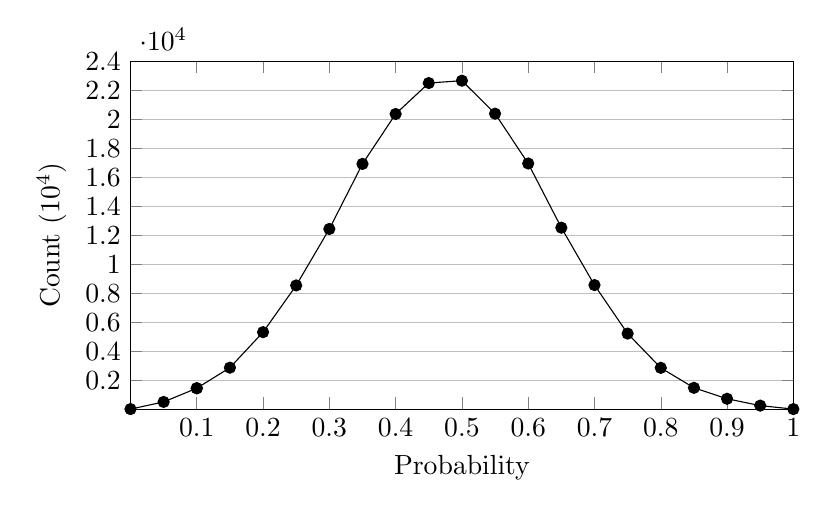
\begin{tikzpicture}
\begin{axis}[
 width=10cm,
   height=6cm,
    xlabel={Probability },
    ylabel={Count ($10^4$)},
    xmin=0, xmax=1.0,
    ymin=0, ymax=24000,
    xtick={.1,.2,.3,.4,.5,.6,.7,.8,.9,1.0},
    ytick={2000,4000,6000,8000,10000,12000,14000,16000,18000,20000,22000,24000},
    legend pos=north east,
    ymajorgrids=true,
    grid style={line width=.2pt,draw=gray!50},
]
 
\addplot[
    solid, every mark/.append style={solid, fill=black}, mark=*
    ]
    coordinates {
		(0,0)
		(.05,495)
		(0.1,1439)
		(0.1 ,1439)
		(0.15,2859)
		(0.2 ,5307)
		(0.25,8531)
		(0.3 ,12426)
		(0.35,16915)
		(0.4 ,20358)
		(0.45,22493)
		(0.5 ,22655)
		(0.55,20380)
		(0.6 ,16943)
		(0.65,12514)
		(0.7 ,8555)
		(0.75,5209)
		(0.8 ,2845)
		(0.85,1468)
		(0.9 ,712)
		(0.95,240)
		(1.0,0)
};
 
\end{axis}
\end{tikzpicture}
%\caption{Probability Distribution for \emph{Mushroom} data set}
\label{result:data_mushroom}
\end{figure}
%\end{document}
        \caption{Probability Distribution for Mushroom ~\cite{dataset} Dataset}
        \label{result:g_dataset_mushroom}
        \end{figure}
        
        \begin{figure}[h]
        \centering
            %%mark = star, diamond, square, otimes
%\documentclass{article}
%\usepackage{pgfplots}
%\usepackage[justification=centering]{caption}
%\pgfplotsset{compat=newest}
%\begin{document}
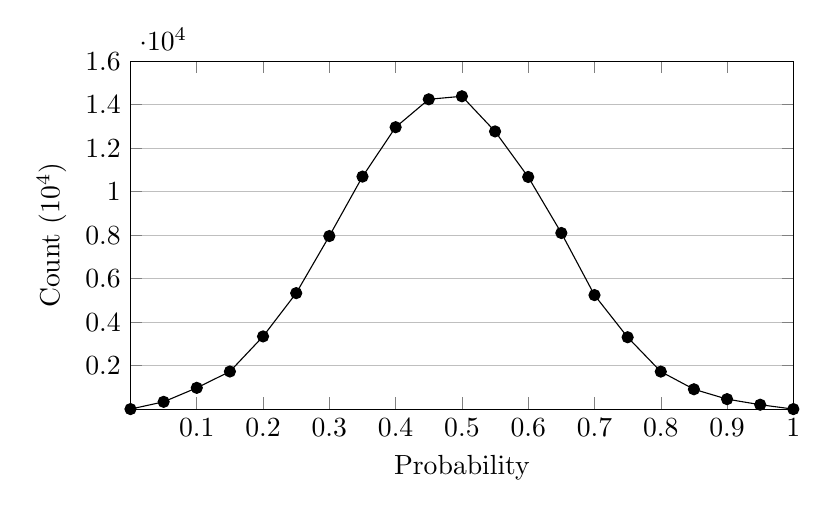
\begin{tikzpicture}
\begin{axis}[
 width=10cm,
   height=6cm,
    xlabel={Probability },
    ylabel={Count ($10^4$)},
    xmin=0, xmax=1.0,
    ymin=0, ymax=16000,
    xtick={.1,.2,.3,.4,.5,.6,.7,.8,.9,1.0},
    ytick={2000,4000,6000,8000,10000,12000,14000,16000},
    legend pos=north east,
    ymajorgrids=true,
    grid style={line width=.2pt,draw=gray!50},
]
 
\addplot[
    solid, every mark/.append style={solid, fill=black}, mark=*
    ]
    coordinates {
			(0,0)
			(0.05,334)
			(0.1,977)
			(0.15,1729)
			(0.2,3342)
			(0.25,5333)
			(0.3,7958)
			(0.35,10692)
			(0.4,12964)
			(0.45,14247)
			(0.5,14386)
			(0.55,12770)
			(0.6,10675)
			(0.65,8099)
			(0.7,5242)
			(0.75,3304)
			(0.8,1724)
			(0.85,912)
			(0.9,458)
			(0.95,201)
			(1,0)

};
 
\end{axis}
\end{tikzpicture}
%\end{document}
        \caption{Probability Distribution for Chess ~\cite{dataset} Dataset}
        \label{result:g_dataset_chess}
        \end{figure}
        \begin{figure}[h]
        \centering
            %%mark = star, diamond, square, otimes
%\documentclass{article}
%\usepackage{pgfplots}
%\usepackage[justification=centering]{caption}
%\pgfplotsset{compat=newest}
%\begin{document}
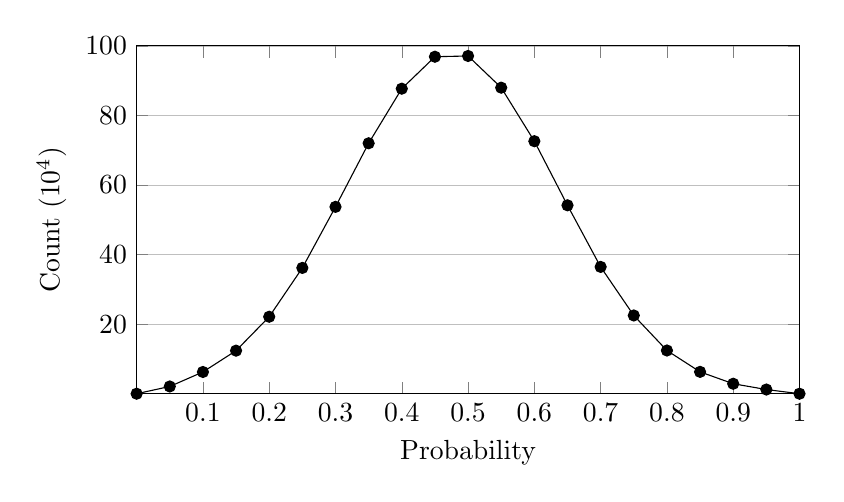
\begin{tikzpicture}
\begin{axis}[
 width=10cm,
   height=6cm,
    xlabel={Probability },
    ylabel={Count ($10^4$)},
    xmin=0, xmax=1.0,
    ymin=0, ymax=100,
    xtick={.1,.2,.3,.4,.5,.6,.7,.8,.9,1.0},
    ytick={20,40,60,80,100},
    legend pos=north east,
    ymajorgrids=true,
    grid style={line width=.2pt,draw=gray!50},
]
 
\addplot[
    solid, every mark/.append style={solid, fill=black}, mark=*
    ]
    coordinates {
		(0			,0	)
		(.05		,2.0856	)
		(0.1 		,6.2495	)
		(0.15		,12.3806	)
		(0.2 		,22.1236	)
		(0.25		,36.1638	)
		(0.3 		,53.7087	)
		(0.35		,71.9860	)
		(0.4 		,87.6780	)
		(0.45		,96.8615	)
		(0.5 		,97.0789	)
		(0.55		,87.9683	)
		(0.6 		,72.5833	)
		(0.65		,54.1544	)
		(0.7 		,36.4540	)
		(0.75		,22.4901	)
		(0.8 		,12.4234	)
		(0.85		,6.2841	)
		(0.9 		,2.8673	)
		(0.95		,1.2048	)
		(1.0		,0	)
};
 
\end{axis}
\end{tikzpicture}
%\end{document}
        \caption{Probability Distribution for Kosarak ~\cite{dataset} Dataset}
        \label{result:g_dataset_kosarak}
        \end{figure}


\subsection{Synthetic Data Set}
For synthetic data sets, we have used T40I10D100K ~\cite{dataset}. It is an IBM generated transaction data set widely used for frequent pattern mining. It is a sparse data set with 100000 transactions and 869 distinct items. For probability assignment to each item, we used the normal distribution for getting the existential probability.
        \begin{figure}[h]
        \centering
            %mark = star, diamond, square, otimes
%\documentclass{article}
%\usepackage{pgfplots}
%\usepackage[justification=centering]{caption}
%\pgfplotsset{compat=newest}
%\begin{document}
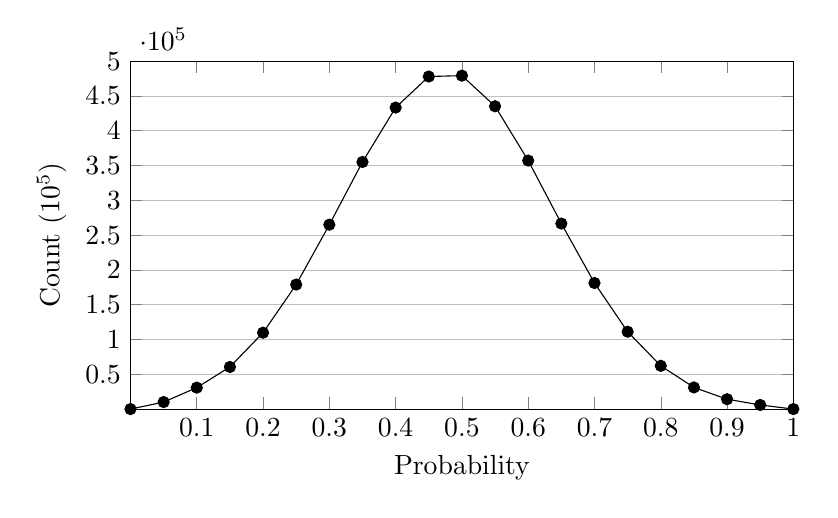
\begin{tikzpicture}
\begin{axis}[
 width=10cm,
   height=6cm,
    xlabel={Probability },
    ylabel={Count ($10^5$)},
    xmin=0, xmax=1.0,
    ymin=0, ymax=500000,
    xtick={.1,.2,.3,.4,.5,.6,.7,.8,.9,1.0},
    ytick={50000,100000,150000,200000,250000,300000,350000,400000,450000,500000},
    legend pos=north east,
    ymajorgrids=true,
    grid style={line width=.2pt,draw=gray!50},
]
 
\addplot[
    solid, every mark/.append style={solid, fill=black}, mark=*
    ]
    coordinates {
			(0,0)
			(0.05,10068)
			(0.1,30825)
			(0.15,60529)
			(0.2,109792)
			(0.25,178975)
			(0.3,265006)
			(0.35,355127)
			(0.4,433334)
			(0.45,477961)
			(0.5,479225)
			(0.55,435233)
			(0.6,357179)
			(0.65,266639)
			(0.7,181169)
			(0.75,111182)
			(0.8,62178)
			(0.85,31116)
			(0.9,14207)
			(0.95,5909)
			(1,0)
};
 
\end{axis}
\end{tikzpicture}
%\end{document}
        \caption{Probability Distribution for T40I10D100K ~\cite{dataset} Dataset}
        \label{result:g_dataset_t10}
        \end{figure}
        
        
\clearpage
\section{Comparison and Analysis}
    In this section we have provided experiment analysis. In the experiment we have focused on (1) correctness of our proposed algorithm and (2) the comparison with existing algorithm SUF-growth ~\cite{suf_growth}. For the extensive experiment we have choose mushroom dataset ~\cite{dataset} and T40I10D100K database. The reason we have choose these two dataset is, mushroom ~\cite{dataset} is real life dataset and dense dataset whereas T40I10D100K ~\cite{dataset} is synthetic and sparse dataset generated by a generator from the IBM Almaden Quest. Table \ref{table:dataset} shows the details the properties for dataset ~\cite{dataset}. Later we have also took chess ~\cite{dataset} for comparison with algorithm. The experimental results have been given in the following subsections.
\subsection{Algorithm Performance Analysis}
	\paragraph{Total Database Size Change Effect}Our experiment shows clearly that our proposed tree construction algorithm \emph{US-tree}, tree mining algorithm \emph{USFP-growth} works nicely with any size of window, batch or transaction size. For Different size of database (transaction count in a tree) this algorithm works extensively. Figure \ref{result:g_m_const_tran} shows the total running time (includes tree construction, mining and false positive reduction) change with the growth of size of mushroom dataset ~\cite{dataset}. Figure \ref{result:g_t10_const_tran} the same characteristic for T40I10D100K dataset ~\cite{dataset}. Figure \ref{result:g_m_const_tran_mem} and figure \ref{result:g_t10_const_tran_mem} shows the total nodes change in a tree while the size of database grows for databases corresponding to mushroom and T40I10D100K database. The growth of the graphs is very much regular. From these graphs it is clearly visible that, with the growth of total transaction the time increases and this certainly proves the scalability of our algorithm. 
		%%%%%%%%%%%%%%%%%%%%%%%%%%%%%%%%%%%%%%%%%%%%%%%%%%%%%%%%%%%%%%%%%%%%%%%%%%%%%%%%%%%%%%%%%%%%%%%%%%%%%%%%%%%%%%%%%%%%%%%%%%%%%%%%%%%%%%%%%%%%%%%%%%%%%%%%%%%%%%%%%%%%%%%%%%%%%%%%%%%%%%%%%%%%%%%%%%%%%%%%%%%%%%%%%%%%%%%%%%%%%
		\begin{figure}[h]
		\centering
			%mark = star, diamond, square, otimes
%\documentclass{article}
%\usepackage{pgfplots}
%\usepackage[justification=centering]{caption}
%\pgfplotsset{compat=newest}
%\begin{document}
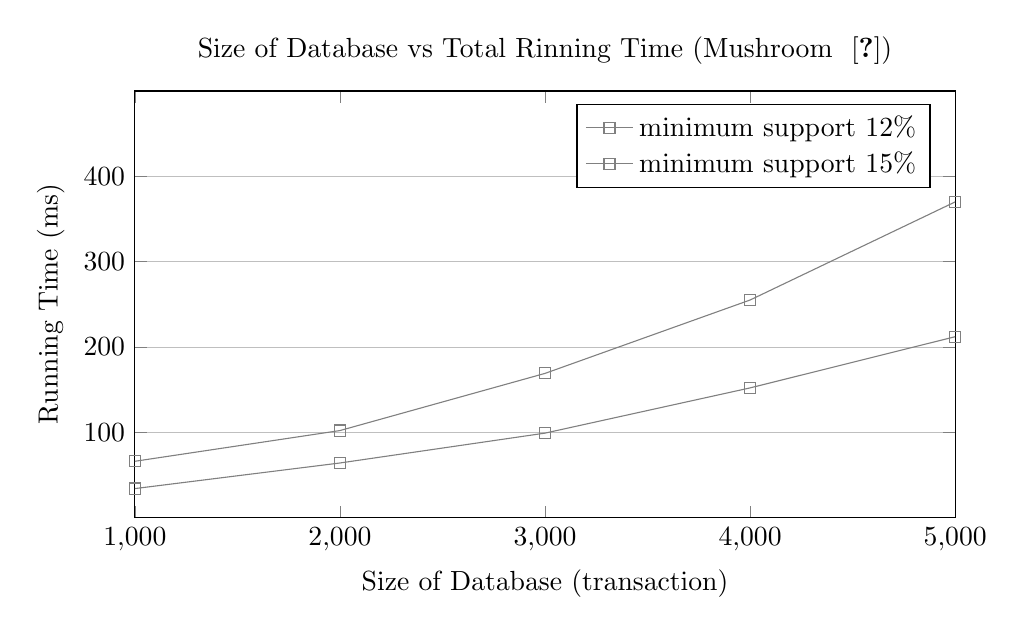
\begin{tikzpicture}
\begin{axis}[
	title={Size of Database vs Total Rinning Time (Mushroom ~\cite{dataset})},
	width=12cm,
	height=7cm,
    xlabel={Size of Database (transaction)},
    ylabel={Running Time (ms)},
    xmin=1000, xmax=5000,
    ymin=0, ymax=500,
    xtick={1000,2000,3000,4000,5000},
    ytick={100,200,300,400},
    legend pos=north east,
    ymajorgrids=true,
    grid style={line width=.2pt,draw=gray!50},
]
 
\addplot[
    solid,color=gray, every mark/.append style={solid, fill=gray}, mark=square
    ]
    coordinates {
		(1000,34)
		(2000,64)
		(3000,99)
		(4000,152)
		(5000,212)

	};
    \addlegendentry{minimum support 12\%}
	
\addplot[
    solid,color=gray, every mark/.append style={solid, fill=gray}, mark=square
    ]
    coordinates {
		(1000,66)
		(2000,102)
		(3000,169)
		(4000,255)
		(5000,370)

	};
    \addlegendentry{minimum support 15\%}

\end{axis}
\end{tikzpicture}
%\end{document}
		\caption{Size of Database vs Running Time for Mushroom Dataset ~\cite{dataset}}
		\label{result:g_m_const_tran}
		\end{figure}
		\begin{figure}[h]
		\centering
			%mark = star, diamond, square, otimes
%\documentclass{article}
%\usepackage{pgfplots}
%\usepackage[justification=centering]{caption}
%\pgfplotsset{compat=newest}
%\begin{document}
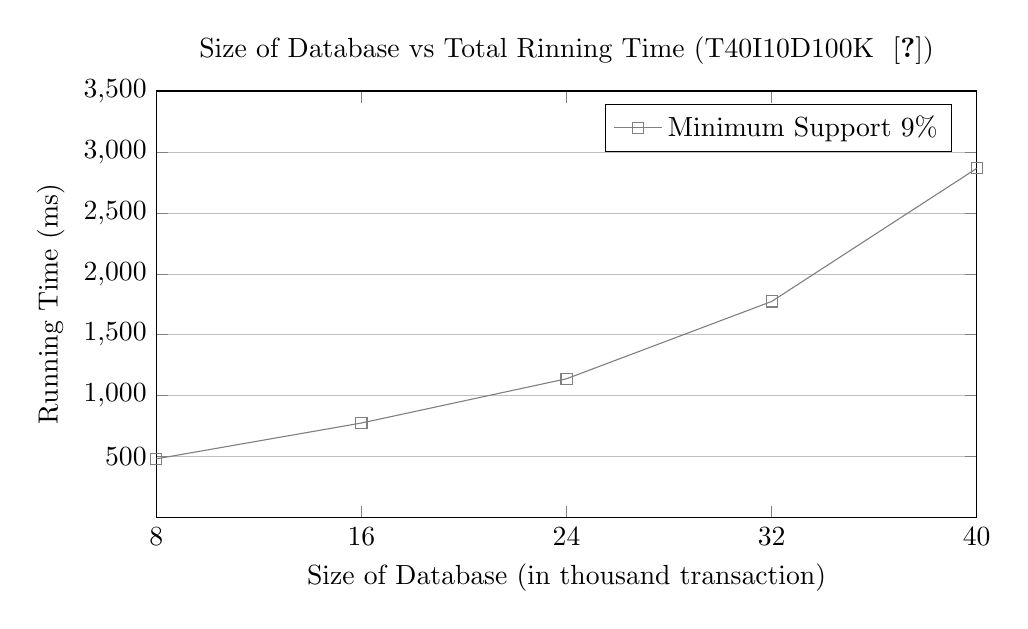
\begin{tikzpicture}
\begin{axis}[
	title={Size of Database vs Total Rinning Time (T40I10D100K ~\cite{dataset})},
	width=12cm,
	height=7cm,
    xlabel={Size of Database (in thousand transaction)},
    ylabel={Running Time (ms)},
    xmin=8, xmax=40,
    ymin=0, ymax=3500,
    xtick={8,16,24,32,40},
    ytick={500,1000,1500,2000,2500,3000,3500},
    legend pos=north east,
    ymajorgrids=true,
    grid style={line width=.2pt,draw=gray!50},
]
 
\addplot[
    solid,color=gray, every mark/.append style={solid, fill=gray}, mark=square
    ]
    coordinates {
			(8,482)
			(16,776)
			(24,1139)
			(32,1773)
			(40,2865)

	};
    \addlegendentry{Minimum Support 9\%}

\end{axis}
\end{tikzpicture}
%\end{document}
		\caption{Size of Database vs Running Time for T40I10D100K Dataset ~\cite{dataset}}
		\label{result:g_t10_const_tran}
		\end{figure}
		%%%%%%%%%%%%%%%%%%%%%%%%%%%%%%%%%%%%%%%%%%%%%%%%%%%%%%%%%%%%%%%%%%%%%%%%%%%%%%%%%%%%%%%%%%%%%%%%%%%%%%%%%%%%%%%%%%%%%%%%%%%%%%%%%%%%%%%%%%%%%%%%%%%%%%%%%%%%%%%%%%%%%%%%%%%%%%%%%%%%%%%%%%%%%%%%%%%%%%%%%%%%%%%%%%%%%%%%%%%%%
		\begin{figure}[h]
		\centering
			%mark = star, diamond, square, otimes
%\documentclass{article}
%\usepackage{pgfplots}
%\usepackage[justification=centering]{caption}
%\pgfplotsset{compat=newest}
%\begin{document}
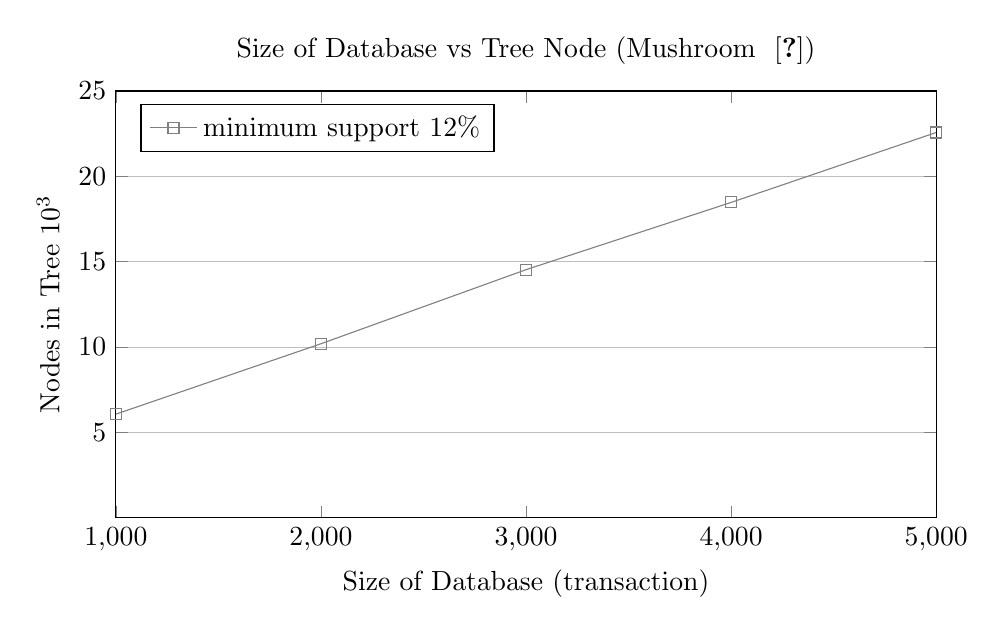
\begin{tikzpicture}
\begin{axis}[
	title={Size of Database vs Tree Node (Mushroom ~\cite{dataset})},
	width=12cm,
	height=7cm,
	xlabel={Size of Database (transaction)},
    ylabel={Nodes in Tree $10^3$},
    xmin=1000, xmax=5000,
    ymin=0, ymax=25,
    xtick={1000,2000,3000,4000,5000},
    ytick={5,10,15,20,25},
    legend pos=north west,
    ymajorgrids=true,
    grid style={line width=.2pt,draw=gray!50},
]
 
\addplot[
    solid,color=gray, every mark/.append style={solid, fill=gray}, mark=square
    ]
    coordinates {
			(1000,6.061 )
			(2000,10.187)
			(3000,14.528)
			(4000,18.469)
			(5000,22.566)


	};
    \addlegendentry{minimum support 12\%}

\end{axis}
\end{tikzpicture}
%\end{document}
		\caption{Size of Database vs Total Nodes in Tree for Mushroom Dataset ~\cite{dataset}}
		\label{result:g_m_const_tran_mem}
		\end{figure}
		\begin{figure}[h]
		\centering
			%mark = star, diamond, square, otimes
%\documentclass{article}
%\usepackage{pgfplots}
%\usepackage[justification=centering]{caption}
%\pgfplotsset{compat=newest}
%\begin{document}
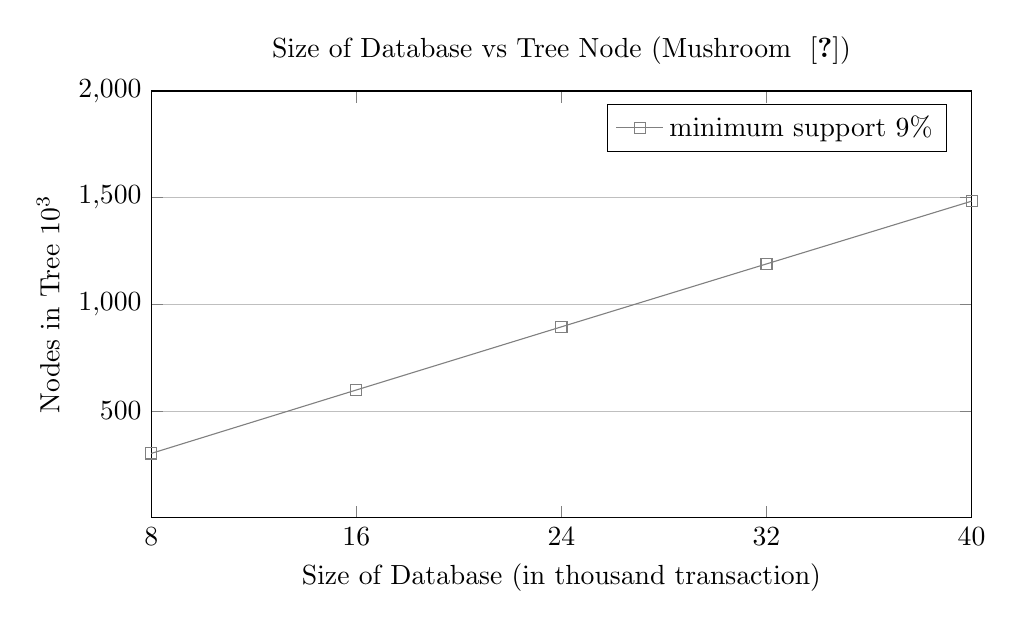
\begin{tikzpicture}
\begin{axis}[
	title={Size of Database vs Tree Node (Mushroom ~\cite{dataset})},
	width=12cm,
	height=7cm,
    xlabel={Size of Database (in thousand transaction)},
    ylabel={Nodes in Tree $10^3$},
    xmin=8, xmax=40,
    ymin=0, ymax=2000,
    xtick={8,16,24,32,40},
    ytick={500,1000,1500,2000},
    legend pos=north east,
    ymajorgrids=true,
    grid style={line width=.2pt,draw=gray!50},
]
 
\addplot[
    solid,color=gray, every mark/.append style={solid, fill=gray}, mark=square
    ]
    coordinates {
			(8,300.856)
			(16,598.221)
			(24,894.225)
			(32,1189.166)
			(40,1483.378)



	};
    \addlegendentry{minimum support 9\%}

\end{axis}
\end{tikzpicture}
%\end{document}
		\caption{Size of Database vs Total Nodes in Tree for T40I10D100K Dataset ~\cite{dataset}}
		\label{result:g_t10_const_tran_mem}
		\end{figure}

	\paragraph{Window Size Change Effect}For window size change effect we have experiment our algorithm in different angle. Experiment shows the window size change effect do not hamper performance and it is consistent. Figure \ref{result:g_m_const_batch} and figure \ref{result:g_t10_const_batch} shows effect of window size change effect on mushroom and T40I10D100K dataset.
		%%%%%%%%%%%%%%%%%%%%%%%%%%%%%%%%%%%%%%%%%%%%%%%%%%%%%%%%%%%%%%%%%%%%%%%%%%%%%%%%%%%%%%%%%%%%%%%%%%%%%%%%%%%%%%%%%%%%%%%%%%%%%%%%%%%%%%%%%%%%%%%%%%%%%%%%%%%%%%%%%%%%%%%%%%%%%%%%%%%%%%%%%%%%%%%%%%%%%%%%%%%%%%%%%%%%%%%%%%%%%
		\begin{figure}[h]
		\centering
			%mark = star, diamond, square, otimes
%\documentclass{article}
%\usepackage{pgfplots}
%\usepackage[justification=centering]{caption}
%\pgfplotsset{compat=newest}
%\begin{document}
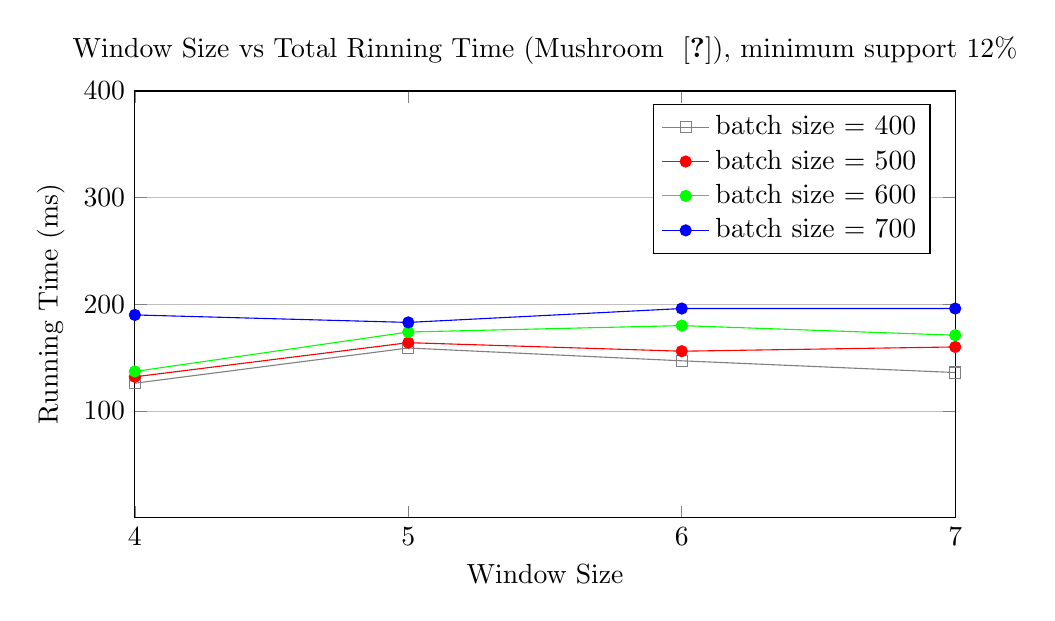
\begin{tikzpicture}
\begin{axis}[
 title={Window Size vs Total Rinning Time (Mushroom ~\cite{dataset}), minimum support 12\%},
 width=12cm,
   height=7cm,
    xlabel={Window Size},
	    ylabel={Running Time (ms)},
    xmin=4, xmax=7,
    ymin=0, ymax=400,
    xtick={4,5,6,7},
    ytick={100,200,300,400},
    legend pos=north east,
    ymajorgrids=true,
    grid style={line width=.2pt,draw=gray!50},
]
 
\addplot[
    solid,color=gray, every mark/.append style={solid, fill=gray}, mark=square
    ]
    coordinates {
			(4,126)			
			(5,159)			
			(6,147)			
			(7,136)
	};
    \addlegendentry{batch size $=$ 400}

	\addplot[
    solid,color=red, every mark/.append style={solid, fill=red}, mark=*
    ]
    coordinates {
			(4,132)			
			(5,164)			
			(6,156)			
			(7,160)
};
    \addlegendentry{batch size $=$ 500}
	

\addplot[
    solid,color=green, every mark/.append style={solid, fill=green}, mark=*
    ]
    coordinates {
			(4,137)			
			(5,174)			
			(6,180)			
			(7,171)
};
    \addlegendentry{batch size $=$ 600}
	
	
\addplot[
    solid,color=blue, every mark/.append style={solid, fill=blue}, mark=*
    ]
    coordinates {
			(4,190)			
			(5,183)			
			(6,196)			
			(7,196)
};
    \addlegendentry{batch size = 700}
\end{axis}
\end{tikzpicture}
%\end{document}
		\caption{Batch Size vs Running Time for Mushroom Dataset ~\cite{dataset}}
		\label{result:g_m_const_batch}
		\end{figure}
		\begin{figure}[h]
		\centering
			%mark = star, diamond, square, otimes
%\documentclass{article}
%\usepackage{pgfplots}
%\usepackage[justification=centering]{caption}
%\pgfplotsset{compat=newest}
%\begin{document}
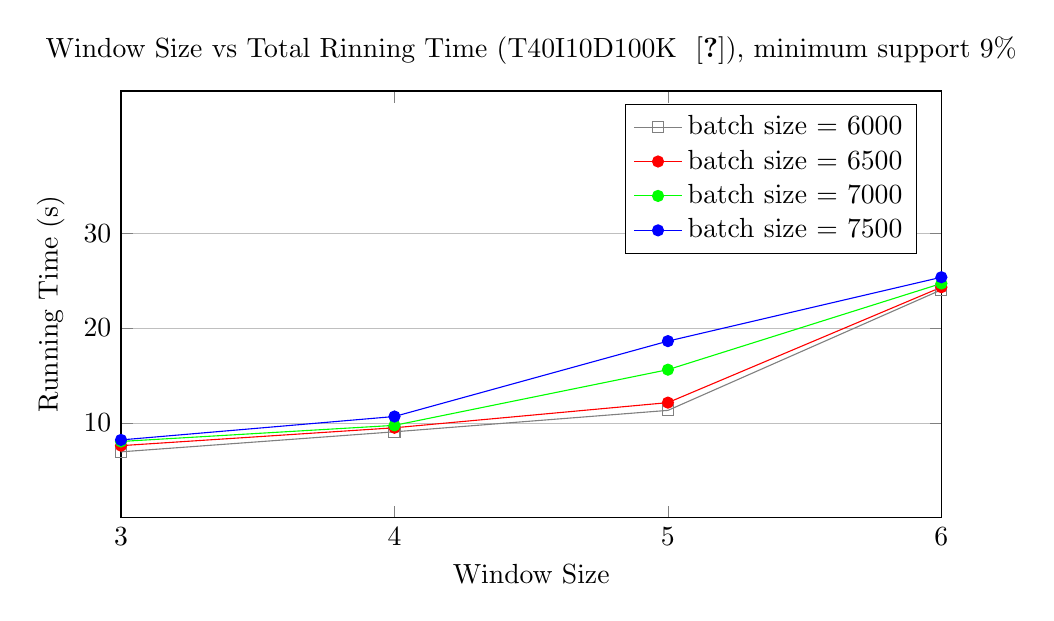
\begin{tikzpicture}
\begin{axis}[
 title={Window Size vs Total Rinning Time (T40I10D100K ~\cite{dataset}), minimum support 9\%},
 width=12cm,
   height=7cm,
    xlabel={Window Size},
    ylabel={Running Time (s)},
    xmin=3, xmax=6,
    ymin=0, ymax=45,
    xtick={3,4,5,6},
    ytick={10,20,30},
    legend pos=north east,
    ymajorgrids=true,
    grid style={line width=.2pt,draw=gray!50},
]
 
\addplot[
    solid,color=gray, every mark/.append style={solid, fill=gray}, mark=square
    ]
    coordinates {
		(3,6.935 )
		(4,9.048 )
		(5,11.308)
		(6,24.026)

	};
    \addlegendentry{batch size $=$ 6000}

	\addplot[
    solid,color=red, every mark/.append style={solid, fill=red}, mark=*
    ]
    coordinates {
		(3,7.587)
		(4,9.473)
		(5,12.126)
		(6,24.299)
};
    \addlegendentry{batch size $=$ 6500}
	

\addplot[
    solid,color=green, every mark/.append style={solid, fill=green}, mark=*
    ]
    coordinates {
		(3,8.030)
		(4,9.729)
		(5,15.602)
		(6,24.690)

};
    \addlegendentry{batch size $=$ 7000}
	
	
\addplot[
    solid,color=blue, every mark/.append style={solid, fill=blue}, mark=*
    ]
    coordinates {
		(3,8.192)
		(4,10.662)
		(5,18.613)
		(6,25.351)
};
    \addlegendentry{batch size $=$ 7500}
\end{axis}
\end{tikzpicture}
%\end{document}
		\caption{Batch Size vs Running Time for T40I10D100K Dataset ~\cite{dataset}}
		\label{result:g_t10_const_batch}
		\end{figure}
		%%%%%%%%%%%%%%%%%%%%%%%%%%%%%%%%%%%%%%%%%%%%%%%%%%%%%%%%%%%%%%%%%%%%%%%%%%%%%%%%%%%%%%%%%%%%%%%%%%%%%%%%%%%%%%%%%%%%%%%%%%%%%%%%%%%%%%%%%%%%%%%%%%%%%%%%%%%%%%%%%%%%%%%%%%%%%%%%%%%%%%%%%%%%%%%%%%%%%%%%%%%%%%%%%%%%%%%		
	\paragraph{Batch Size Change Effect}Like batch change effect we also experimented for batch size change effect.For changing batch size in different volume the result we find is consistent. For constant window and variable batches we have simulated our proposed algorithms. Figure \ref{result:g_m_const_batch} and figure \ref{result:g_t10_const_batch} shows effect of batch size change effect on mushroom and T40I10D100K dataset.
		\begin{figure}[h]
		\centering
			%mark = star, diamond, square, otimes
%\documentclass{article}
%\usepackage{pgfplots}
%\usepackage[justification=centering]{caption}
%\pgfplotsset{compat=newest}
%\begin{document}
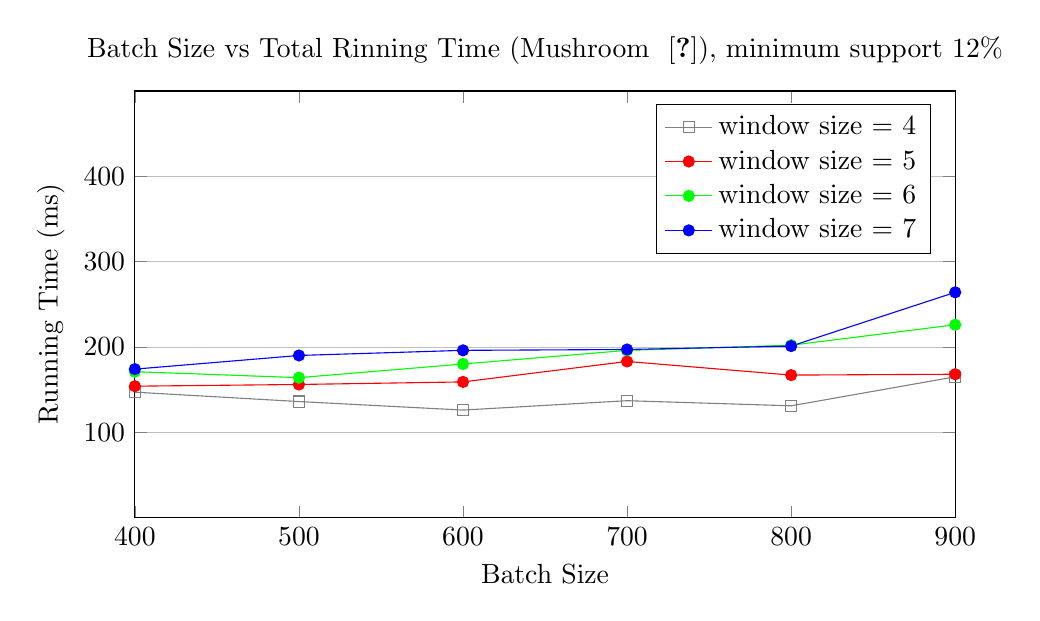
\begin{tikzpicture}
\begin{axis}[
 title={Batch Size vs Total Rinning Time (Mushroom ~\cite{dataset}), minimum support 12\%},
 width=12cm,
   height=7cm,
    xlabel={Batch Size},
    ylabel={Running Time (ms)},
    xmin=400, xmax=900,
    ymin=0, ymax=500,
    xtick={400,500,600,700,800,900},
    ytick={100,200,300,400},
    legend pos=north east,
    ymajorgrids=true,
    grid style={line width=.2pt,draw=gray!50},
]
 
\addplot[
    solid,color=gray, every mark/.append style={solid, fill=gray}, mark=square
    ]
    coordinates {
			(400,147)
			(500,136)
			(600,126)
			(700,137)
			(800,131)
			(900,165)
	};
    \addlegendentry{window size $=$ 4}

	\addplot[
    solid,color=red, every mark/.append style={solid, fill=red}, mark=*
    ]
    coordinates {
			(400,154)
			(500,156)
			(600,159)
			(700,183)
			(800,167)
			(900,168)
};
    \addlegendentry{window size $=$ 5}
	

\addplot[
    solid,color=green, every mark/.append style={solid, fill=green}, mark=*
    ]
    coordinates {
			(400,171)
			(500,164)
			(600,180)
			(700,196)
			(800,202)
			(900,226)
};
    \addlegendentry{window size $=$ 6}
	
	
\addplot[
    solid,color=blue, every mark/.append style={solid, fill=blue}, mark=*
    ]
    coordinates {
			(400,174)
			(500,190)
			(600,196)
			(700,197)
			(800,201)
			(900,264)
};
    \addlegendentry{window size = 7}
\end{axis}
\end{tikzpicture}
%\end{document}
		\caption{Window Size vs Running Time for Mushroom Dataset ~\cite{dataset}}
		\label{result:g_m_const_win}
		\end{figure}
		\begin{figure}[h]
		\centering
			%mark = star, diamond, square, otimes
%\documentclass{article}
%\usepackage{pgfplots}
%\usepackage[justification=centering]{caption}
%\pgfplotsset{compat=newest}
%\begin{document}
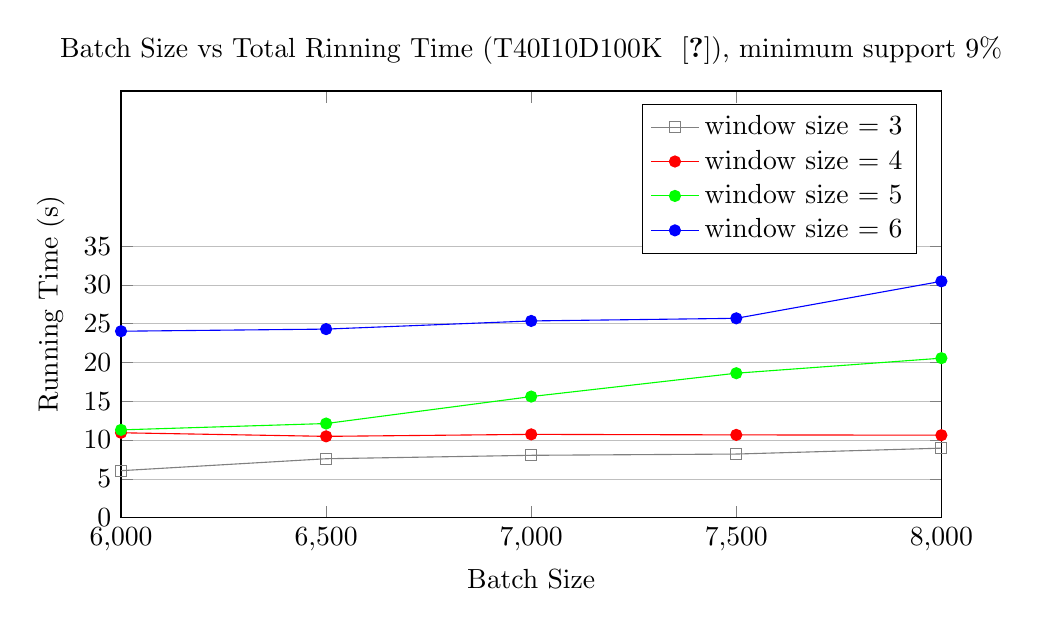
\begin{tikzpicture}
\begin{axis}[
 title={Batch Size vs Total Rinning Time (T40I10D100K ~\cite{dataset}), minimum support 9\%},
 width=12cm,
   height=7cm,
    xlabel={Batch Size},
    ylabel={Running Time (s)},
    xmin=6000, xmax=8000,
    ymin=0, ymax=55,
    xtick={6000,6500,7000,7500,8000},
    ytick={0,5,10,15,20,25,30,35},
    legend pos=north east,
    ymajorgrids=true,
    grid style={line width=.2pt,draw=gray!50},
]
 
\addplot[
    solid,color=gray, every mark/.append style={solid, fill=gray}, mark=square
    ]
    coordinates {
		(6000,6.048)
		(6500,7.587 )
		(7000,8.030 )
		(7500,8.192 )
		(8000,8.951 )
	};
    \addlegendentry{window size $=$ 3}

	\addplot[
    solid,color=red, every mark/.append style={solid, fill=red}, mark=*
    ]
    coordinates {
		(6000,10.935)
		(6500,10.473)
		(7000,10.729)
		(7500,10.662)
		(8000,10.625)

};
    \addlegendentry{window size $=$ 4}
	

\addplot[
    solid,color=green, every mark/.append style={solid, fill=green}, mark=*
    ]
    coordinates {
		(6000,11.308)
		(6500,12.126)
		(7000,15.602)
		(7500,18.613)
		(8000,20.552)

};
    \addlegendentry{window size $=$ 5}
	
	
\addplot[
    solid,color=blue, every mark/.append style={solid, fill=blue}, mark=*
    ]
    coordinates {
		(6000,24.026)
		(6500,24.299)
		(7000,25.351)
		(7500,25.690)
		(8000,30.460)

};
    \addlegendentry{window size $=$ 6}
\end{axis}
\end{tikzpicture}
%\end{document}
		\caption{Window Size vs Running Time for T40I10D100K Dataset ~\cite{dataset}}
		\label{result:g_t10_const_win}
		\end{figure}
		%%%%%%%%%%%%%%%%%%%%%%%%%%%%%%%%%%%%%%%%%%%%%%%%%%%%%%%%%%%%%%%%%%%%%%%%%%%%%%%%%%%%%%%%%%%%%%%%%%%%%%%%%%%%%%%%%%%%%%%%%%%%%%%%%%%%%%%%%%%%%%%%%%%%%%%%%%%%%%%%%%%%%%%%%%%%%%%%%%%%%%%%%%%%%%%%%%%%%%%%%%%%%%%%%%%%%%%%%%%%%
\clearpage
%%%%%%%%%%%%%%%%%%%%%%%%%%%%%%%%%%%%%%%%%%%%%%%%%%%%%%%%%%%%%%%%%%%%%%%%%%%%%%%%%%%%%%%%%%%%%%%%%%%%%%%%%%%%%%%%%%%%%%%%%%%%%%%%%%%%%%%%%%%%%%%%%%%%%%%%%%%%%%%%%%%%%%%%%%%%%%%%%%%%%%%%%%%%%%%%%%%%%%%%%%%%%%%%%%%%%%%%%%%%		
\subsection{Comparison With Existing Approaches}
Here now we have compared our proposed approach with existing system. We have choose SUF-growth ~\cite{suf_growth}  for comparison. This algorithm is perfectly fit for uncertain stream data mining. UF-streaming also designed for mining frequent patterns from uncertain stream but in ~\cite{suf_growth} it has been proved that in all criteria (running time, memory and correctness) SUF-growth ~\cite{suf_growth} is better than UF-streaming ~\cite{suf_growth}. We have experimented for both running time performance and memory efficiency. The result has described below:
	\subsubsection{Running Time Comparison}
	Run time comparison has been experimented and the in the result we found is consistent and we have gained run time efficiency for both dense and sparse dataset. For mushroom dataset our approach's total tree construction time , total mining time and total time has been compared with SUF-growth ~\cite{suf_growth}'s tree construction time and mining time and total time. Figure \ref{result:g_m_tree_construction_total}, figure \ref{result:g_m_mining_total} and figure \ref{result:g_m_total} shows the result graph. As mushroom is a dense database we gain much more in run time. For dense characteristic the constructed \emph{US-tree} is very much compact and more over when mining compact tree the mining time surprisingly decreases that effect the total time. Figure \ref{result:g_t10_tree_construction_total}, figure \ref{result:g_t10_mining_total} and figure \ref{result:g_t10_total} shows same comparison for T40I10D100K dataset ~\cite{dataset}. The graphs shows that our algorithm works correctly for sparse dataset too. Figure \ref{result:g_chess_tree_construction_total}, figure \ref{result:g_chess_mining_total} and figure \ref{result:g_chess_total} shows tree construction time, mining time and total time for chess dataset. This one is dense dataset and the result is consistent, efficient and also scalable.
			\begin{figure}[h]
			\centering
				%%mark = star, diamond, square, otimes
%\documentclass{article}
%\usepackage{pgfplots}
%\usepackage[justification=centering]{caption}
%\pgfplotsset{compat=newest}
%\begin{document}
\begin{figure}
\centering

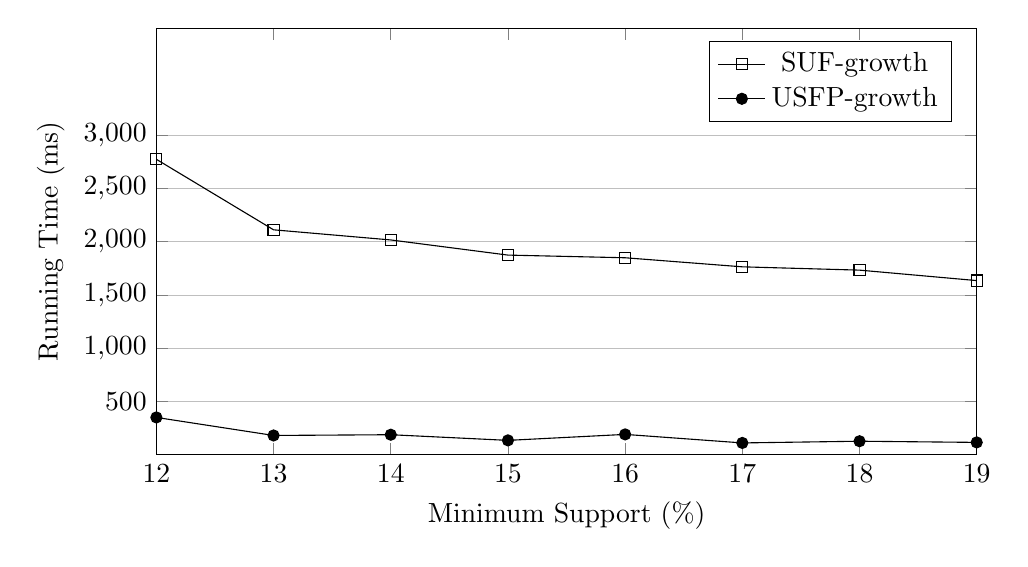
\begin{tikzpicture}
\begin{axis}[
 width=12cm,
   height=7cm,
    xlabel={Minimum Support (\%) },
    ylabel={Running Time (ms)},
    xmin=12, xmax=19,
    ymin=0, ymax=4000,
    xtick={12,13,14,15,16,17,18,19},
    ytick={500,1000,1500,2000,2500,3000},
    legend pos=north east,
    ymajorgrids=true,
    grid style={line width=.2pt,draw=gray!50},
]
 
\addplot[
    solid, every mark/.append style={solid, fill=gray}, mark=square
    ]
    coordinates {
	(12,2771)
	(13,2110)
	(14,2015)
	(15,1873)
	(16,1848)
	(17,1763)
	(18,1732)
	(19,1634)
	};
    \addlegendentry{SUF-growth}
\addplot[
    solid, every mark/.append style={solid, fill=black}, mark=*
    ]
    coordinates {
	(12,351)
	(13,182)
	(14,189)
	(15,136)
	(16,192)
	(17,112)
	(18,128)
	(19,117)
};
    \addlegendentry{USFP-growth}
 
\end{axis}
\end{tikzpicture}
%\caption{Total Tree Construction Time vs Minimum Suppport (\%) \\(Window Size = 4, Frame Size = 650) for mushroom database}
\label{result:mushroom_tree_total}
\end{figure}
%\end{document}
			\caption{Total Tree Construction Time vs Minimum Support (\%) for Mushroom Dataset ~\cite{dataset}}
			\label{result:g_m_tree_construction_total}
			\end{figure}
			
			\begin{figure}[h]
			\centering
				%mark = star, diamond, square, otimes
\documentclass{article}
\usepackage{pgfplots}
\usepackage[justification=centering]{caption}
\pgfplotsset{compat=newest}
\begin{document}
\begin{figure}
\centering

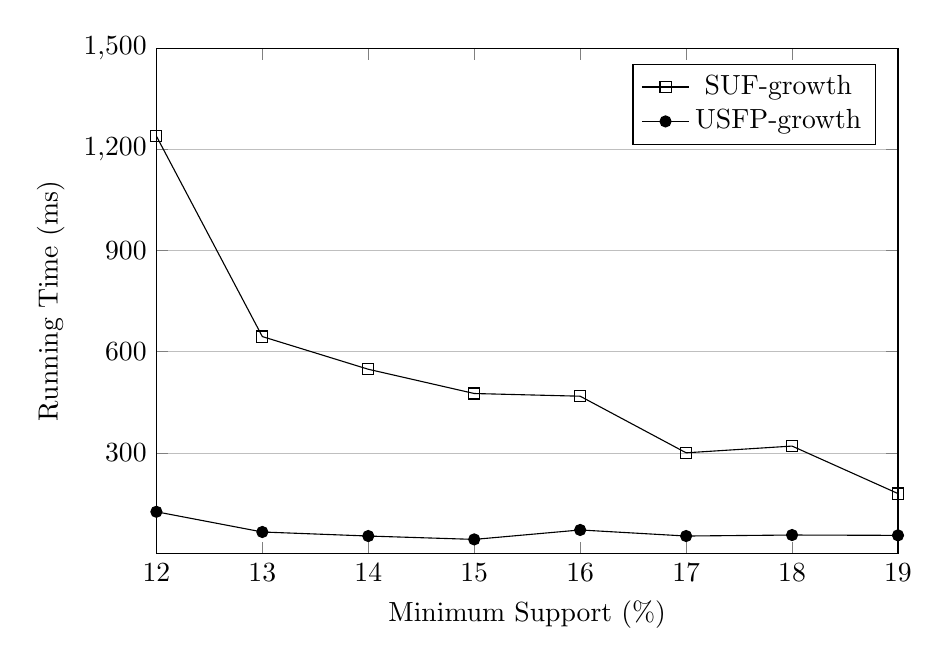
\begin{tikzpicture}
\begin{axis}[
 width=11cm,
   height=8cm,
    xlabel={Minimum Support (\%) },
    ylabel={Running Time (ms)},
    xmin=12, xmax=19,
    ymin=0, ymax=1500,
    xtick={12,13,14,15,16,17,18,19},
    ytick={300,600,900,1200,1500,2000},
    legend pos=north east,
    ymajorgrids=true,
    grid style={line width=.2pt,draw=gray!50},
]
 
\addplot[
    solid, every mark/.append style={solid, fill=gray}, mark=square
    ]
    coordinates {
	(12,1240)
	(13,645)
	(14,548)
	(15,476)
	(16,468)
	(17,300)
	(18,320)
	(19,179)
};
    \addlegendentry{SUF-growth}
\addplot[
    solid, every mark/.append style={solid, fill=black}, mark=*
    ]
    coordinates {
	(12,125)
	(13,65 )
	(14,53 )
	(15,43 )
	(16,71 )
	(17,53 )
	(18,56 )
	(19,55 )
};
    \addlegendentry{USFP-growth}
 
\end{axis}
\end{tikzpicture}
\caption{Total Tree Mining vs Minimum Suppport (\%) \\(Window Size = 4, Frame Size = 650) for mushroom database}
\label{result:mushroom_total}
\end{figure}
\end{document}
			\caption{Total Tree Mining Time vs Minimum Support (\%) for Mushroom Dataset ~\cite{dataset}}
			\label{result:g_m_mining_total}
			\end{figure}
			\begin{figure}[h]
			\centering
				%%mark = star, diamond, square, otimes
%\documentclass{article}
%\usepackage{pgfplots}
%\usepackage[justification=centering]{caption}
%\pgfplotsset{compat=newest}
%\begin{document}
\begin{figure}
\centering

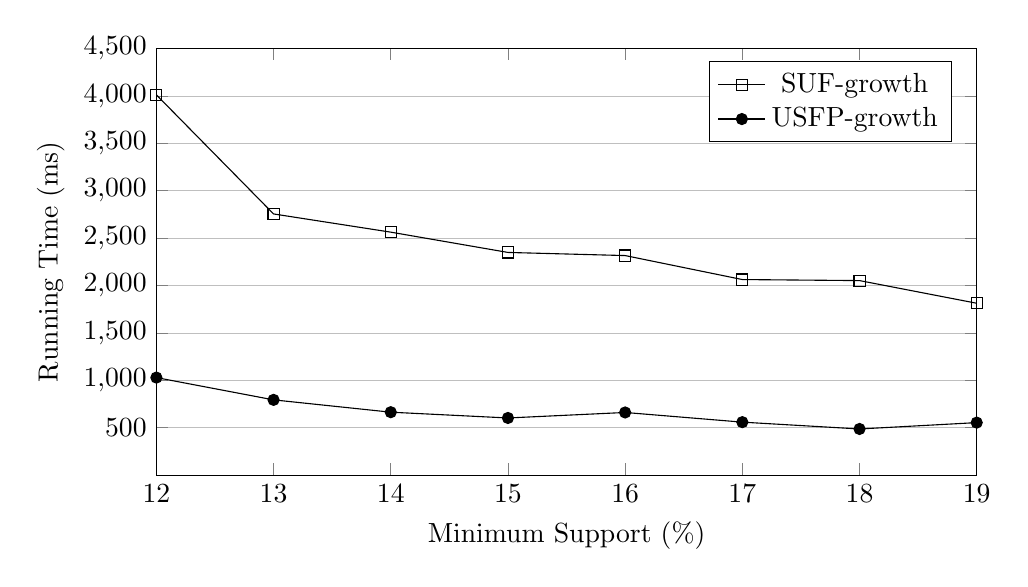
\begin{tikzpicture}
\begin{axis}[
 width=12cm,
   height=7cm,
    xlabel={Minimum Support (\%) },
    ylabel={Running Time (ms)},
    xmin=12, xmax=19,
    ymin=0, ymax=4500,
    xtick={12,13,14,15,16,17,18,19},
    ytick={500,1000,1500,2000,2500,3000,3500,4000,4500},
    legend pos=north east,
    ymajorgrids=true,
    grid style={line width=.2pt,draw=gray!50},
]
 
\addplot[
    solid, every mark/.append style={solid, fill=gray}, mark=square
    ]
    coordinates {
	(12,4011)
	(13,2755)
	(14,2563)
	(15,2349)
	(16,2316)
	(17,2063)
	(18,2052)
	(19,1813)
};
    \addlegendentry{SUF-growth}
\addplot[
    solid, every mark/.append style={solid, fill=black}, mark=*
    ]
    coordinates {
	(12,1029)
	(13,794)
	(14,664)
	(15,603)
	(16,661)
	(17,559)
	(18,487)
	(19,554)
};
    \addlegendentry{USFP-growth}
 
\end{axis}
\end{tikzpicture}
caption{Total Time (Tree Construction + Mining + False Positive Reduction) vs Minimum Suppport (\%) ( Window Size = 4, Frame Size = 650 ) for mushroom database}
\label{result:mushroom_total}
\end{figure}
%\end{document}
			\caption{Running Time vs Minimum Support (\%) for Mushroom Dataset ~\cite{dataset}}
			\label{result:g_m_total}
			\end{figure}
			\begin{figure}[h]
			\centering
				%%mark = star, diamond, square, otimes
%\documentclass{article}
%\usepackage{pgfplots}
%\usepackage[justification=centering]{caption}
%\pgfplotsset{compat=newest} 	title={\parbox{\linewidth}{\centering Total Tree Construction Time vs Minimum Suppport (\%) for T40I10D100K ~\cite{dataset}, Window Size = 5, Frame Size = 7000}},
%\begin{document}
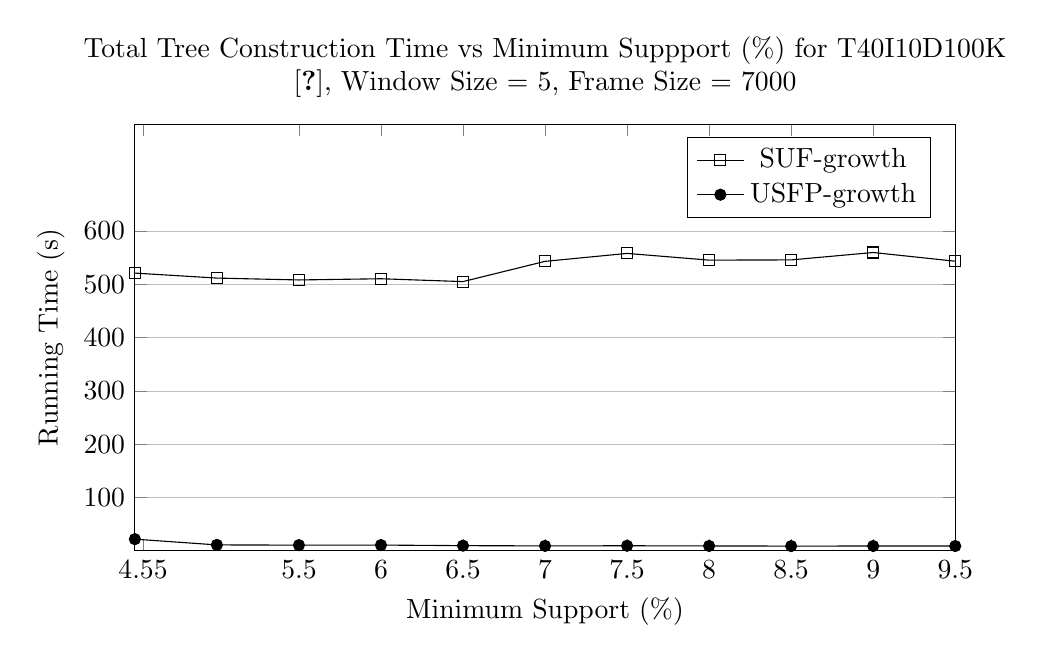
\begin{tikzpicture}
	\begin{axis}[
	title={\parbox{\linewidth}{\centering Total Tree Construction Time vs Minimum Suppport (\%) for T40I10D100K ~\cite{dataset}, Window Size = 5, Frame Size = 7000}},
	width=12cm,
	height=7cm,
    xlabel={Minimum Support (\%) },
    ylabel={Running Time (s)},
    xmin=4.5, xmax=9.5,
    ymin=0, ymax=800,
    xtick={4.55,5.5,6,6.5,7,7.5,8,8.5,9,9.5},
    ytick={100,200,300,400,500,600},
    legend pos=north east,
    ymajorgrids=true,
    grid style={line width=.2pt,draw=gray!50},
]
 
\addplot[
    solid, every mark/.append style={solid, fill=gray}, mark=square
    ]
    coordinates {
			(4.5,520.723)
			(5  ,511.365)
			(5.5,507.854)
			(6  ,510.12 )
			(6.5,504.767)
			(7  ,542.742)
			(7.5,557.633)
			(8  ,545.039)
			(8.5,545.444)
			(9  ,559.335)
			(9.5,542.996)

	};
    \addlegendentry{SUF-growth}
\addplot[
    solid, every mark/.append style={solid, fill=black}, mark=*
    ]
    coordinates {
		(4.5,21.814)
		(5  ,11.035)
		(5.5,10.601)
		(6  ,10.723)
		(6.5,9.646 )
		(7  ,9.177 )
		(7.5,9.427 )
		(8  ,9.092 )
		(8.5,8.8   )
		(9  ,8.95  )
		(9.5,8.883 )

};
    \addlegendentry{USFP-growth}
 
\end{axis}
\end{tikzpicture}
%\end{document}
			\caption{Total Tree Construction Time vs Minimum Support (\%) for T40I10D100K Dataset ~\cite{dataset}}
			\label{result:g_t10_tree_construction_total}
			\end{figure}
			
			\begin{figure}[h]
			\centering
				%%%mark = star, diamond, square, otimes
%\documentclass{article}
%\usepackage{pgfplots}
%\usepackage[justification=centering]{caption}
%\pgfplotsset{compat=newest}
%\begin{document}
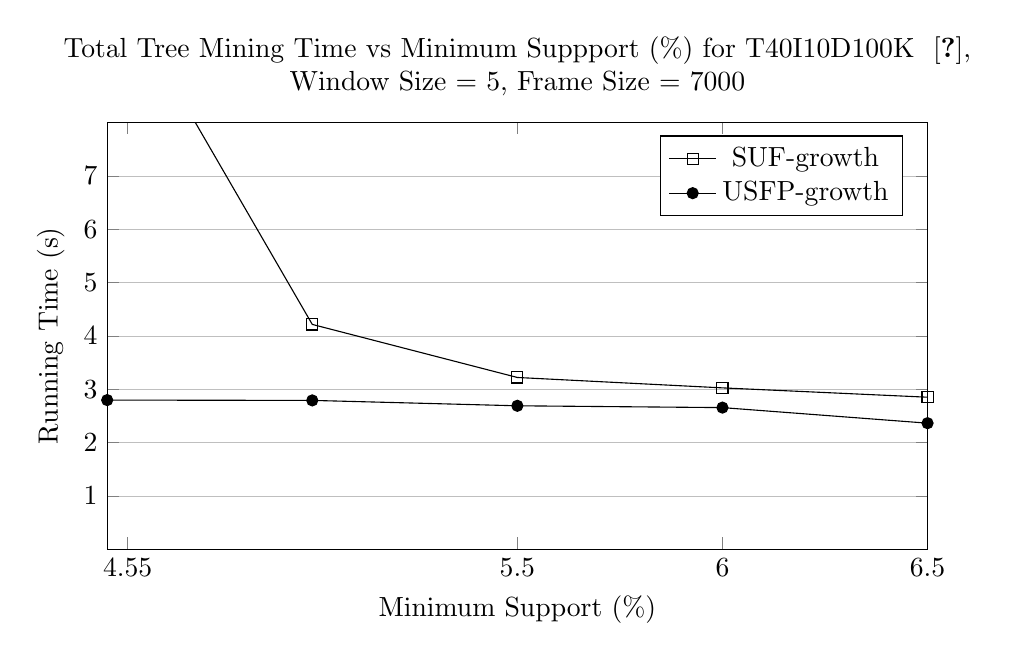
\begin{tikzpicture}
\begin{axis}[
	title={\parbox{\linewidth}{\centering Total Tree Mining Time vs Minimum Suppport (\%) for T40I10D100K ~\cite{dataset}, Window Size = 5, Frame Size = 7000}},
	width=12cm,
	height=7cm,
    xlabel={Minimum Support (\%) },
    ylabel={Running Time (s)},
    xmin=4.5, xmax=6.5,
    ymin=0, ymax=8,
    xtick={4.55,5.5,6,6.5},
    ytick={1,2,3,4,5,6,7},
    legend pos=north east,
    ymajorgrids=true,
    grid style={line width=.2pt,draw=gray!50},
]
 
\addplot[
    solid, every mark/.append style={solid, fill=gray}, mark=square
    ]
    coordinates {
			(4.5,10.856)
			(5  ,4.216 )
			(5.5,3.221 )
			(6  ,3.026 )
			(6.5,2.851 )


};
    \addlegendentry{SUF-growth}
\addplot[
    solid, every mark/.append style={solid, fill=black}, mark=*
    ]
    coordinates {
			(4.5,  2.797)
			(5  , 2.791)
			(5.5,2.69 )
			(6  ,2.656 )
			(6.5,2.364 )


};
    \addlegendentry{USFP-growth}
 
\end{axis}
\end{tikzpicture}
%\end{document}
			\caption{Total Tree Mining Time vs Minimum Support (\%) for T40I10D100K Dataset ~\cite{dataset}}
			\label{result:g_t10_mining_total}
			\end{figure}
			
			\begin{figure}[h]
			\centering
				%%%mark = star, diamond, square, otimes
%\documentclass{article}
%\usepackage{pgfplots}
%\usepackage[justification=centering]{caption}
%\pgfplotsset{compat=newest}
%\begin{document}
\begin{figure}[!h]
\centering

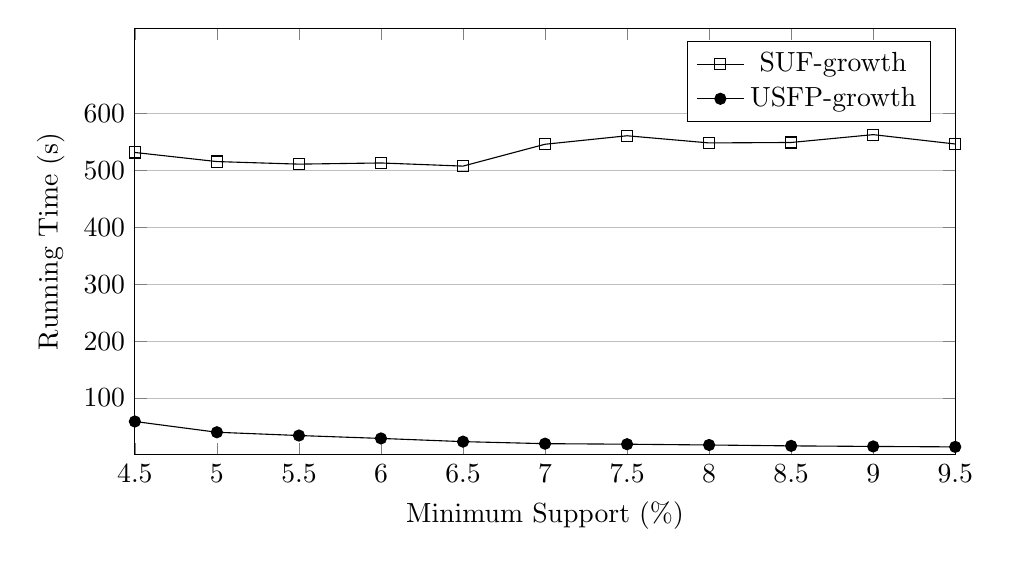
\begin{tikzpicture}
\begin{axis}[
 width=12cm,
   height=7cm,
    xlabel={Minimum Support (\%) },
    ylabel={Running Time (s)},
    xmin=4.5, xmax=9.5,
    ymin=0, ymax=750,
    xtick={4.5,5,5.5,6,6.5,7,7.5,8,8.5,9,9.5},
    ytick={100,200,300,400,500,600},
    legend pos=north east,
    ymajorgrids=true,
    grid style={line width=.2pt,draw=gray!50},
]
 
\addplot[
    solid, every mark/.append style={solid, fill=gray}, mark=square
    ]
    coordinates {
			(4.5,531.579)
			(5  ,515.581)
			(5.5,511.075)
			(6  ,513.146)
			(6.5,507.618)
			(7  ,546.032)
			(7.5,560.952)
			(8  ,548.354)
			(8.5,549.139)
			(9  ,562.928)
			(9.5,546.47 )

};
    \addlegendentry{SUF-growth}
\addplot[
    solid, every mark/.append style={solid, fill=black}, mark=*
    ]
    coordinates {
			(4.5,58.652)
			(5  ,39.735)
			(5.5,33.993)
			(6  ,28.892)
			(6.5,23.262)
			(7  ,19.669)
			(7.5,18.735)
			(8  ,17.355)
			(8.5,15.785)
			(9  ,14.803)
			(9.5,14.013)

};
    \addlegendentry{USFP-growth}
 
\end{axis}
\end{tikzpicture}
\caption{Total Time (Tree Construction + Mining + False Positive Reduction) vs Minimum Suppport (\%) \\(Window Size = 5, Frame Size = 7000) for T40I10D100K database}
\label{result:t10_total}
\end{figure}
%\end{document}
			\caption{Running Time vs Minimum Support (\%) for T40I10D100K Dataset ~\cite{dataset}}
			\label{result:g_t10_total}
			\end{figure}
	
			\begin{figure}[h]
			\centering
				%%mark = star, diamond, square, otimes
%\documentclass{article}
%\usepackage{pgfplots}
%\usepackage[justification=centering]{caption}
%\pgfplotsset{compat=newest}
%\begin{document} 
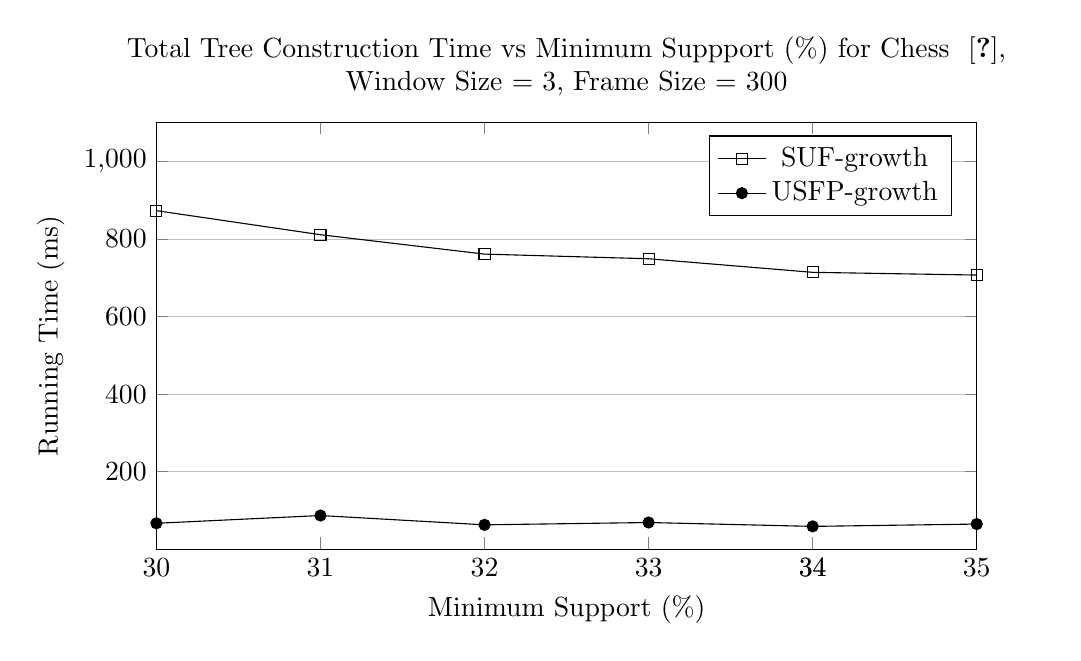
\begin{tikzpicture}
\begin{axis}[
	title={\parbox{\linewidth}{\centering Total Tree Construction Time vs Minimum Suppport (\%) for Chess ~\cite{dataset}, Window Size = 3, Frame Size = 300}},
	width=12cm,
	height=7cm,
    xlabel={Minimum Support (\%) },
    ylabel={Running Time (ms)},
    xmin=30, xmax=35,
    ymin=0, ymax=1100,
    xtick={30,31,32,33,34,34,35},
    ytick={200,400,600,800,1000},
    legend pos=north east,
    ymajorgrids=true,
    grid style={line width=.2pt,draw=gray!50},
]
 
\addplot[
    solid, every mark/.append style={solid, fill=gray}, mark=square
    ]
    coordinates {
			(30,873)
			(31,811)
			(32,761)
			(33,749)
			(34,714)
			(35,707)

	};
    \addlegendentry{SUF-growth}
\addplot[
    solid, every mark/.append style={solid, fill=black}, mark=*
    ]
    coordinates {
			(30,67)
			(31,87)
			(32,63)
			(33,69)
			(34,59)
			(35,65)

};
    \addlegendentry{USFP-growth}
 
\end{axis}
\end{tikzpicture}
%\end{document}
			\caption{Total Tree Construction Time vs Minimum Support (\%) for Chess Dataset ~\cite{dataset}}
			\label{result:g_chess_tree_construction_total}
			\end{figure}
			
			\begin{figure}[h]
			\centering
				%%mark = star, diamond, square, otimes
%\documentclass{article}
%\usepackage{pgfplots}
%\usepackage[justification=centering]{caption}
%\pgfplotsset{compat=newest}
%\begin{document}
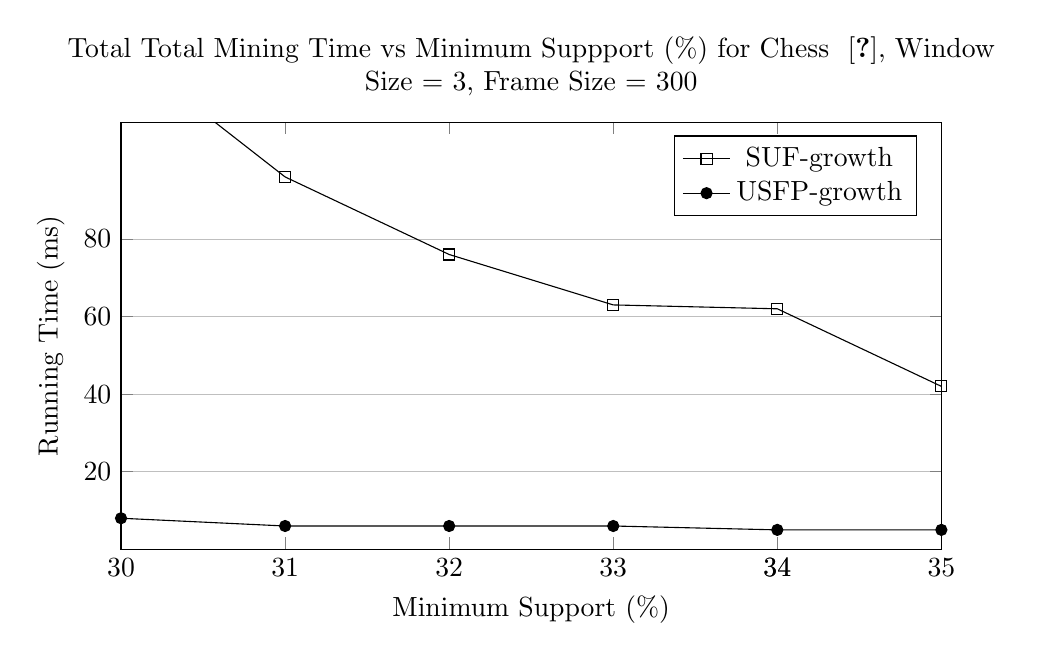
\begin{tikzpicture}
\begin{axis}[
	title={\parbox{\linewidth}{\centering Total Total Mining Time vs Minimum Suppport (\%) for Chess ~\cite{dataset}, Window Size = 3, Frame Size = 300}},
	width=12cm,
	height=7cm,
    xlabel={Minimum Support (\%) },
    ylabel={Running Time (ms)},
    xmin=30, xmax=35,
    ymin=0, ymax=110,
    xtick={30,31,32,33,34,34,35},
    ytick={20,40,60,80},
    legend pos=north east,
    ymajorgrids=true,
    grid style={line width=.2pt,draw=gray!50},
]
 
\addplot[
    solid, every mark/.append style={solid, fill=gray}, mark=square
    ]
    coordinates {
			(30,129)
			(31,96)
			(32,76)
			(33,63)
			(34,62)
			(35,42)

};
    \addlegendentry{SUF-growth}
\addplot[
    solid, every mark/.append style={solid, fill=black}, mark=*
    ]
    coordinates {
			(30,8)
			(31,6)
			(32,6)
			(33,6)
			(34,5)
			(35,5)

};
    \addlegendentry{USFP-growth}
 
\end{axis}
\end{tikzpicture}
%\end{document}
			\caption{Total Tree Mining Time vs Minimum Support (\%) for Chess Dataset ~\cite{dataset}}
			\label{result:g_chess_mining_total}
			\end{figure}
			
			\begin{figure}[h]
			\centering
				%%mark = star, diamond, square, otimes
%\documentclass{article}
%\usepackage{pgfplots}
%\usepackage[justification=centering]{caption}
%\pgfplotsset{compat=newest}
%\begin{document}
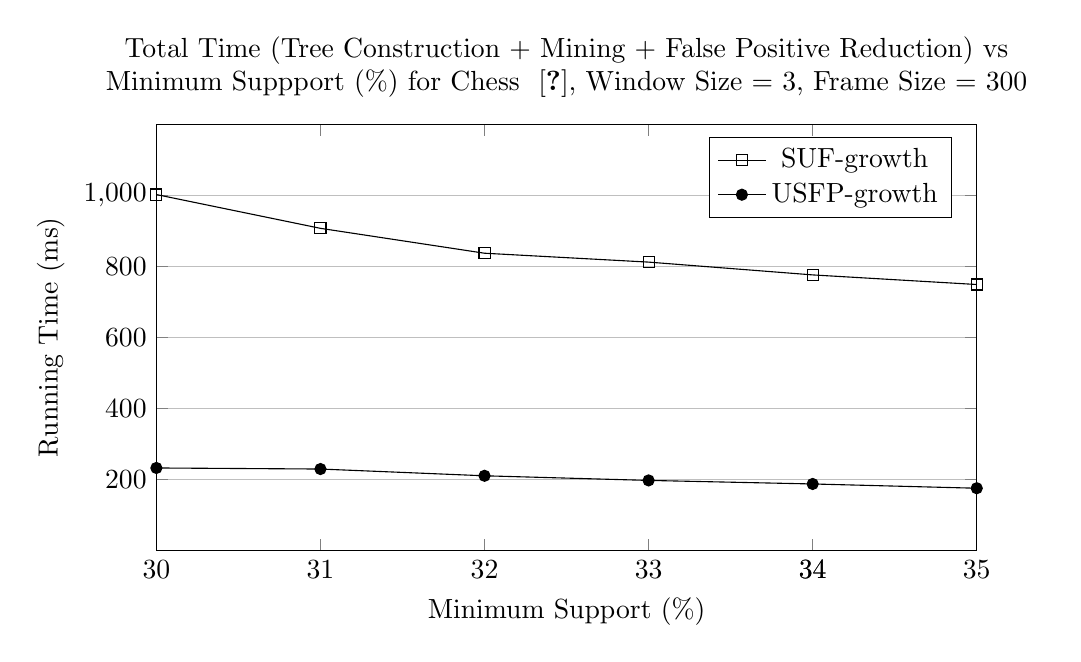
\begin{tikzpicture}
\begin{axis}[
	title={\parbox{\linewidth}{\centering Total Time (Tree Construction + Mining + False Positive Reduction) vs Minimum Suppport (\%) for Chess ~\cite{dataset}, Window Size = 3, Frame Size = 300}},
	width=12cm,
	height=7cm,
    xlabel={Minimum Support (\%) },
    ylabel={Running Time (ms)},
    xmin=30, xmax=35,
    ymin=0, ymax=1200,
    xtick={30,31,32,33,34,34,35},
    ytick={200,400,600,800,1000},
    legend pos=north east,
    ymajorgrids=true,
    grid style={line width=.2pt,draw=gray!50},
]
 
\addplot[
    solid, every mark/.append style={solid, fill=gray}, mark=square
    ]
    coordinates {
			(30,1002)
			(31,907)
			(32,837)
			(33,812)
			(34,776)
			(35,749)
};
    \addlegendentry{SUF-growth}
\addplot[
    solid, every mark/.append style={solid, fill=black}, mark=*
    ]
    coordinates {
			(30,233)
			(31,230)
			(32,211)
			(33,198)
			(34,188)
			(35,176)

};
    \addlegendentry{USFP-growth}
 
\end{axis}
\end{tikzpicture}
%\end{document}
			\caption{Running Time vs Minimum Support (\%) for Chess Dataset ~\cite{dataset}}
			\label{result:g_chess_total}
			\end{figure}
\clearpage
	\subsubsection{Memory Comparison}
		As our proposed \emph{US-tree} have capability to share nodes more than \emph{SUF-growth} ~\cite{dataset}, we get much more gain in memory. The experimental result also indicates that very clearly. Figure \ref{result:g_m_memory_node} shows the memory comparison on mushroom dataset. Mushroom is dense database so we get  much more gain in memory. The graph clearly shows that with the increase of total transaction in the tree gives the much more gain. For chess dataset the the compactness of tree is also very impressive as this dataset is also compact (figure \ref{result:g_chess_memory_node}) the Dense dataset have more scope to share nodes more. Figure \ref{result:g_t10_memory_node} also shows that in T40I10D100K database we also gain the memory optimization. As the database is sparse, we get the memory gain less then dense one.
			\begin{figure}[h]
			\centering
				%mark = star, diamond, square, otimes
%\documentclass{article}
%\usepackage{pgfplots}
%\usepackage[justification=centering]{caption}
%\pgfplotsset{compat=newest}
%\begin{document}
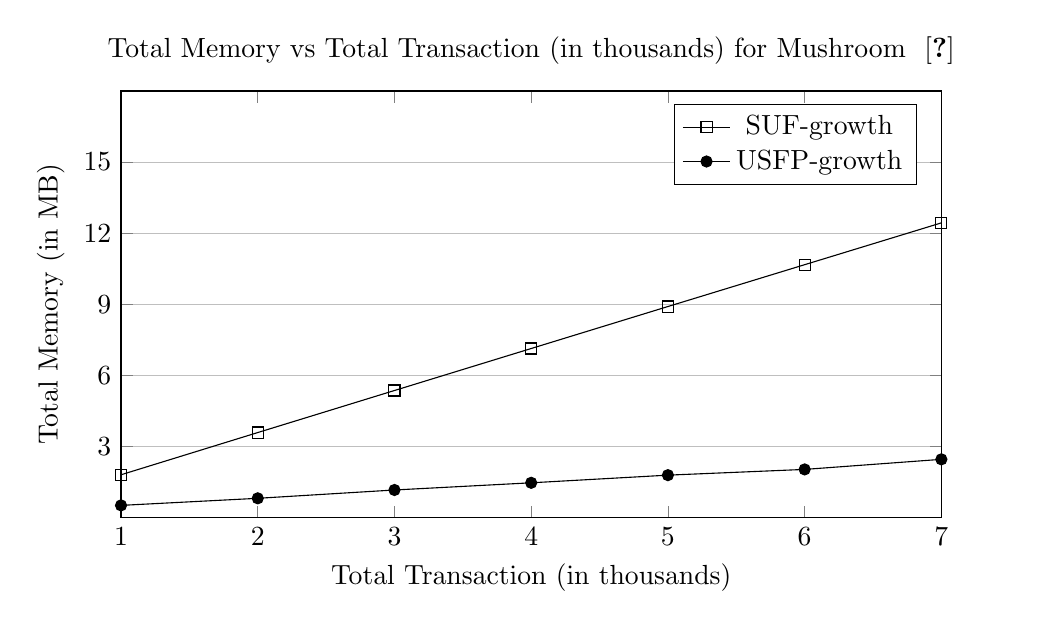
\begin{tikzpicture}
\begin{axis}[
	title={\parbox{\linewidth}{\centering Total Memory vs Total Transaction (in thousands) for Mushroom ~\cite{dataset}}},
	width=12cm,
	height=7cm,
    xlabel={Total Transaction (in thousands) },
    ylabel={Total Memory (in MB) },
    xmin=1, xmax=7,
    ymin=0, ymax=18,
    xtick={1,2,3,4,5,6,7},
    ytick={3,6,9,12,15},
    legend pos=north east,
    ymajorgrids=true,
    grid style={line width=.2pt,draw=gray!50},
]
 
\addplot[
    solid, every mark/.append style={solid, fill=gray}, mark=square
    ]
    coordinates {
			(1,1.807  )
			(2,3.588  )
			(3,5.362  )
			(4,7.134     )
			(5,8.905  )
			(6,10.670 )
			(7,12.434  )



	};
    \addlegendentry{SUF-growth}
\addplot[
    solid, every mark/.append style={solid, fill=black}, mark=*
    ]
    coordinates {
			(1,.5152  )
			(2,.814  )
			(3,1.165 )
			(4,1.468 )
			(5,1.791  )
			(6,2.033 )
			(7,2.458 )


};
    \addlegendentry{USFP-growth}
 
\end{axis}
\end{tikzpicture}
%\end{document}
			\caption{Avg Tree Node per window vs Frame Size for Mushroom Dataset ~\cite{dataset}}
			\label{result:g_m_memory_node}
			\end{figure}
			
			\begin{figure}[h]
			\centering
				%mark = star, diamond, square, otimes
%\documentclass{article}
%\usepackage{pgfplots}
%\usepackage[justification=centering]{caption}
%\pgfplotsset{compat=newest}
%\begin{document}
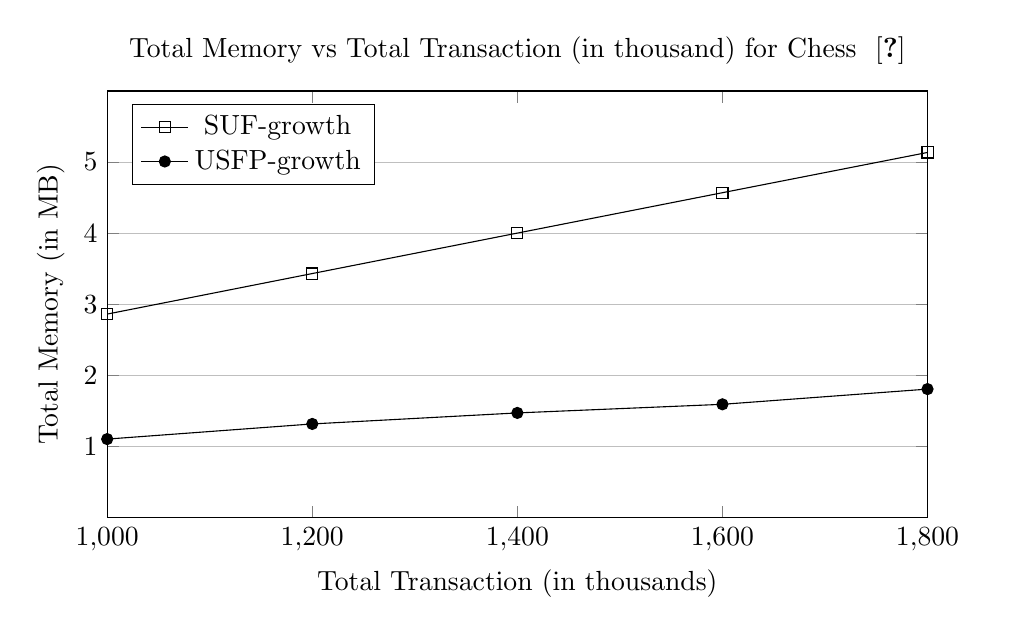
\begin{tikzpicture}
\begin{axis}[
	title={\parbox{\linewidth}{\centering Total Memory vs Total Transaction (in thousand) for Chess ~\cite{dataset}}},
	width=12cm,
	height=7cm,
    xlabel={Total Transaction (in thousands) },
    ylabel={Total Memory (in MB) },
    xmin=1000, xmax=1800,
    ymin=0, ymax=6,
    xtick={600,800,1000,1200,1400,1600,1800},
    ytick={1,2,3,4,5},
    legend pos=north west,
    ymajorgrids=true,
    grid style={line width=.2pt,draw=gray!50},
]
 
\addplot[
    solid, every mark/.append style={solid, fill=gray}, mark=square
    ]
    coordinates {
			(600,	1.720)
			(800,	2.291)
			(1000,	2.862)
			(1200,	3.432)
			(1400,	4.001)
			(1600,	4.569)
            (1800,	5.135)



	};
    \addlegendentry{SUF-growth}
\addplot[
    solid, every mark/.append style={solid, fill=black}, mark=*
    ]
    coordinates {
			(600,	0.681 )
			(800,	0.865 )
			(1000,	1.104 )
			(1200,	1.317 )
			(1400,	1.472 )
			(1600,	1.593 )
            (1800,	1.807 )


};
    \addlegendentry{USFP-growth}
 
\end{axis}
\end{tikzpicture}
%\end{document}
			\caption{Avg Tree Node per window vs Frame Size for Chess Dataset ~\cite{dataset}}
			\label{result:g_chess_memory_node}
			\end{figure}
			
			\begin{figure}[h]
				%%%mark = star, diamond, square, otimes
%\documentclass{article}
%\usepackage{pgfplots}
%\usepackage[justification=centering]{caption}
%\pgfplotsset{compat=newest}
%\begin{document}
\begin{figure}
\centering

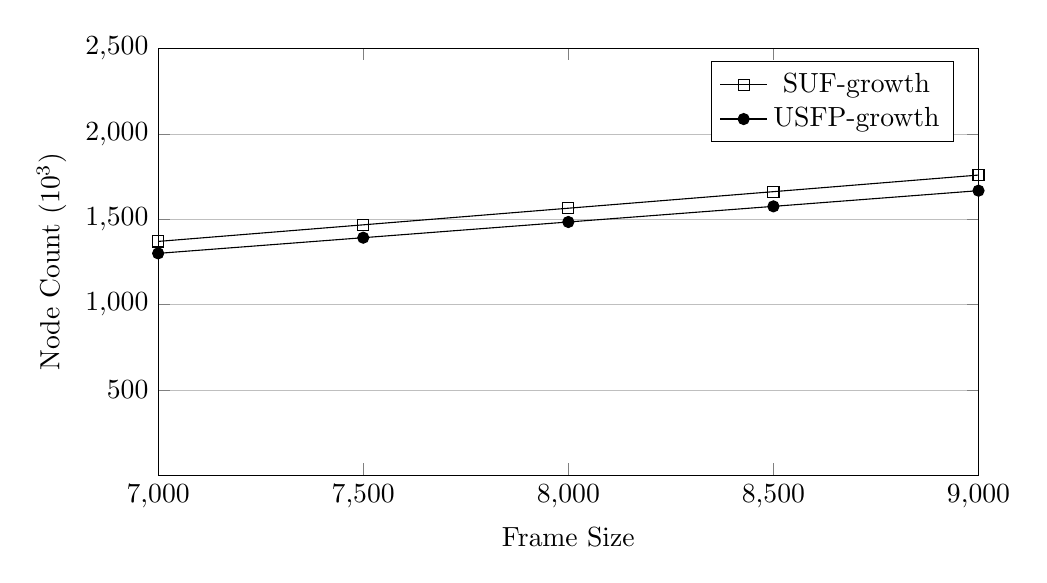
\begin{tikzpicture}
\begin{axis}[
 width=12cm,
   height=7cm,
    xlabel={Frame Size },
    ylabel={Node Count ($10^3$)},
    xmin=7000, xmax=9000,
    ymin=0, ymax=2500,
    xtick={7000,7500,8000,8500,9000},
    ytick={500,1000,1500,2000,2500},
    legend pos=north east,
    ymajorgrids=true,
    grid style={line width=.2pt,draw=gray!50},
]
 
\addplot[
    solid, every mark/.append style={solid, fill=gray}, mark=square
    ]
    coordinates {
			(7000,1369.555 )
			(7500,1466.766 )
			(8000,1564.122 )
			(8500,1661.100 )
			(9000,1758.412 )
			(9500,1855.734 )

	};
    \addlegendentry{SUF-growth}
\addplot[
    solid, every mark/.append style={solid, fill=black}, mark=*
    ]
    coordinates {
					(7000,1299.510)
		(7500,1391.388)
		(8000,1483.378)
		(8500,1574.984)
		(9000,1666.912)
		(9500,1758.773)

};
    \addlegendentry{USFP-growth}
 
\end{axis}
\end{tikzpicture}
\caption{Total Tree Node vs Frame Size (Window Size = 5) for T40I10D100K database}
\label{result:t10_total_mem_node}
\end{figure}
%\end{document}
			\caption{Avg Tree Node per window vs Frame Size for T40I10D100K Dataset ~\cite{dataset}}
			\label{result:g_t10_memory_node}
			\end{figure}
		

\clearpage
\section{Summary}
In summary, our proposed \emph{US-tree}, construction \emph{USFP-growth} mining algorithm is very correct, efficient, the scalable algorithm that works fine in any configuration (minimum support, window size, batch size). For dense dataset (both real and synthetic) this is very efficient. For sparse dataset, this also gives us gain both in memory and in running time. The \emph{U\textsuperscript{cap}} value gives much more benefit to share nodes in the \emph{US-tree}. The compactness of \emph{US-tree} is surprisingly noticeable. Mining compact \emph{US-tree} gives the main surprise in the running time. The \emph{USFP-growth} mining algorithm works nicely without generating no false negatives and a little amount of false positives that can efficiently be removed using the false positive reduction technique.
%
%\end{document}